\section*{Petri Nets}
% \begin{frame}
%   \frametitle{Petri Nets}
%   \centering
%   \hspace{-2cm}
%   \includegraphics[width=10cm]{images/"petrinet - petri-complete"}
% \end{frame}

% \begin{frame}
%   \frametitle{Petri Nets}
%   \hspace*{-.5cm}\makebox1[\linewidth][c]{%
%   \begin{columns}
%     \begin{column}{0.6\linewidth}
%       \includegraphics[width=5cm]{images/"petrinet - graphic-primitives"}
%     \end{column}
%     \begin{column}{0.6\linewidth}
%       \includegraphics[width=6cm]{images/"csd - petrinet-metamodel"}
%     \end{column}
%   \end{columns}
%   }
% \end{frame}


\section{Design}
\begin{frame}
  \centering
  \hspace{-1cm}
  \huge
  \red{Design}
\end{frame}

\begin{frame}
  \frametitle{Architecture Idea}
  \includesvg[width=12cm]{images/"component - architecture-idea"}
\end{frame}

\begin{frame}
  \frametitle{Implemented Module}
  \centering
  \hspace{-1cm}
  \includesvg[width=10cm]{images/"component - config-interpreter"}
\end{frame}


\begin{frame}
  \frametitle{Metamodel}
  \centering
  \hspace{-1cm}
  \includesvg[width=13cm]{images/"csd - metamodel"}
\end{frame}


\begin{frame}
  \frametitle{}
  \centering
  \hspace{-1cm}
  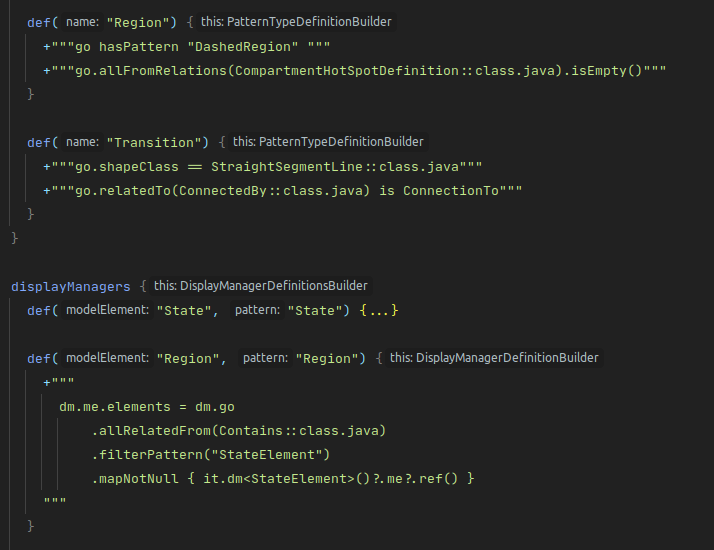
\includegraphics[width=8.5cm]{images/dsl-strings}
\end{frame}

% \begin{frame}
%   \frametitle{Render Metamodel}
%   \centering
%   \hspace{-1cm}
%   \includesvg[width=5cm]{images/"csd - rendersyntax"}
% \end{frame}

% \begin{frame}
%   \frametitle{Abstract Syntax Metamodel}
%   \centering
%   \hspace{-1cm}
%   \includesvg[width=6cm]{images/"csd - abstractsyntax"}
% \end{frame}

\begin{frame}
  \frametitle{Concrete Syntax Metamodel}
  \hspace{-1cm}
  \centering
  \includesvg[width=10cm]{images/"csd - concretesyntax"}
\end{frame}


\begin{frame}
  \frametitle{Making Metamodels Aware of Concrete Syntax}

  \centering
  \hspace{-1cm}
  \includesvg[width=10cm]{images/"presentation - dm-sync"}
\end{frame}


\begin{frame}
  \frametitle{Sync token count}
  \texttt{\textbf{context} PlaceDM \\
  \textbf{inv}: self.me.tokens = self.go.tokens->count()}

  \centering
  \hspace{-1cm}
  \includesvg[width=10cm]{images/"presentation - dm-sync-text"}
\end{frame}

\begin{frame}
  \frametitle{Making Metamodels Aware of Concrete Syntax}

  \centering
  \hspace{-1cm}
  \includesvg[width=10cm]{images/"presentation - dm-sync-question"}
\end{frame}

% \begin{frame}
%   \frametitle{Place Syncing}
%   \begin{itemize}
%     \item token count of abstract element equals Elements\\ contained by graphic object
%   \end{itemize}
% \end{frame}

\begin{frame}
  \frametitle{}

  \centering
  \hspace*{-1.5cm}
  \begin{tabular}{m{11.5cm}  m{5cm}}
    \includesvg[width=10cm]{images/"presentation - my-fondement"}
     &
    % \vspace{2.5cm}
    \includesvg[width=2cm]{images/"labeled-place"}
  \end{tabular}
\end{frame}

% \begin{frame}
%   \frametitle{Graph Querying in CouchEdit}
%   \vspace{.5cm}
%   \texttt{queryService.allRelatedFrom(\textbf{GO},\textbf{Contains}::class.java)}

%   \vspace{1cm}
%   \texttt{\textbf{GO}.allRelatedFrom(\textbf{Contains}::class.java)}

%   \vspace{-2.5cm}
%   \hspace*{-1.5cm}
%   \begin{tabular}{m{10cm}  m{5cm}}
%     \includesvg[width=10cm]{images/"presentation - kind-0"}
%      &
%     \vspace{2.5cm}
%     \includesvg[width=2cm]{images/"petrinet - token-check"}
%   \end{tabular}
% \end{frame}



\begin{frame}
  \frametitle{DisplayManagers}
  \hspace{-1cm}
  \centering
  \includesvg[width=10cm]{images/"presentation - concrete-blur-1"}
\end{frame}


% \begin{frame}
%   \frametitle{DisplayManagers}
%   \hspace{-1cm}
%   \includegraphics[width=10cm]{images/"csd - fondement-dm"}
% \end{frame}


% \begin{frame}
%   \frametitle{Place DisplayManager}
%   \hspace{-1cm}
%   \includegraphics[width=10cm]{images/"csd - fondement-example"}
% \end{frame}


% \begin{frame}
%   \frametitle{Place DisplayManager in CouchEdit}
%   \hspace{-1cm}
%   \includegraphics[width=10cm]{images/"presentation - my-fondement"}
% \end{frame}


\begin{frame}[fragile]
  \frametitle{Place Pattern}
  % \vspace{-1cm}
  % \begin{lstlisting}
  %   go.shape is Circle

  % go.allRelatedTo(Contains).isEmpty()
  % \end{lstlisting}

  \hspace*{-1.5cm}
  \begin{tabular}{m{7cm}  m{5cm}}
    \begin{itemize}
      \setlength\itemsep{.6cm}
      \item GO has shape Circle
      % \item GO fillColor is not black
      \item GO is not Contained by another GO
    \end{itemize}
     &
    \vspace{-.5cm}
    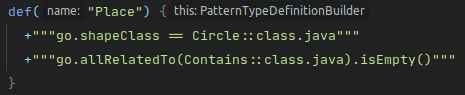
\includegraphics[width=7cm]{images/place-pattern}
  \end{tabular}
\end{frame}

\begin{frame}
  \frametitle{Recognition of Place Pattern}
  % \vspace{-2.5cm}
  \hspace*{-1.5cm}
  \begin{tabular}{m{10cm}  m{5cm}}
    \includesvg[width=10cm]{images/"presentation - kind-0"}
     &
    \vspace{2.5cm}
    \includesvg[width=2cm]{images/"petrinet - token-check"}
  \end{tabular}
\end{frame}

\begin{frame}
  \frametitle{Recognition of Place Pattern}
  \hspace*{-1.5cm}
  \begin{tabular}{m{10cm}  m{5cm}}
    \includesvg[width=10cm]{images/"presentation - kind-1"}
     &
    \vspace{2.5cm}
    \includesvg[width=2cm]{images/"petrinet - token-check"}
  \end{tabular}
\end{frame}

\begin{frame}
  \frametitle{DisplayManager System}
  \hspace{-1cm}
  \centering
  \includesvg[width=10cm]{images/"presentation - concrete-blur-2"}
\end{frame}

\begin{frame}
  \frametitle{PlaceDM is Added}
  \hspace*{-1.5cm}
  \begin{tabular}{m{10cm}  m{5cm}}
    \includesvg[width=10cm]{images/"presentation - kind-2"}
     &
    \vspace{2.5cm}
    \includesvg[width=2cm]{images/"petrinet - token-check"}
  \end{tabular}
\end{frame}

% \begin{frame}
%   \frametitle{Syncing Token Count}
%   \centering
%   \hspace{-1cm}  
%   \includegraphics[width=3cm]{images/"petrinet - token-check"}
% \end{frame}

% \begin{frame}[fragile]
%   \frametitle{Syncing Token count}
% %   \vspace*{-2cm}
% %   \begin{lstlisting}
% % dm.me.tokens = 
% %   dm.go
% %     .allRelatedFrom(Contains)
% %     .count()
% %   \end{lstlisting}

% \end{frame}

\begin{frame}
  \frametitle{Syncing Token count}

  Tokens of model element == \\number graphic objects contained by graphic representative

  \vspace{1cm}
  \centering
  \hspace{-1cm}
  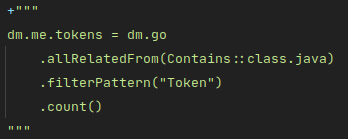
\includegraphics[width=8cm]{images/token-sync}

\end{frame}


\begin{frame}
  \frametitle{Syncing Token count}
  \hspace*{-1.5cm}
  \begin{tabular}{m{10cm}  m{5cm}}
    \includesvg[width=10cm]{images/"presentation - syncing-1"}
     &
    \vspace{2.5cm}
    \includesvg[width=2cm]{images/"petrinet - token-check"}
  \end{tabular}
\end{frame}

% \begin{frame}
%   \frametitle{Syncing Token count}
%   \hspace{-1cm}
%   \includegraphics[width=10cm]{images/"presentation - syncing-2"}
% \end{frame}


% \begin{frame}
%   \frametitle{Syncing outgoing Transitions}

%   \centering
%   \hspace{-1cm}
%   \includegraphics[width=3cm]{images/"petrinet - outgoing-example-1"}
% \end{frame}


% \begin{frame}
%   \frametitle{Syncing outgoing Transitions}
%   \hspace{-1cm}
%   \includegraphics[width=10cm]{images/"presentation - syncing-3"}
% \end{frame}


% \begin{frame}[fragile]
%   \frametitle{Syncing outgoing Transitions}
%   \vspace*{-1cm}
%   \begin{lstlisting}
% dm.me.outgoing = 
%   dm.go
%     .allToRelations(ConnectionEnd)
%     .filter { rel -> !rel.isEndConnection }
%     .map { rel -> rel.getA() }
%     .flatMap { line -> line
%       .allFromRelations(ConnectionEnd) }
%     .filter { rel -> rel.isEndConnection }
%     .map { rel -> rel.getB() } 
%     .map { go -> go.dm.me }
%   \end{lstlisting}
% \end{frame}

% \begin{frame}
%   \frametitle{Syncing outgoing Transitions}
%   \hspace{-1cm}
%   \includegraphics[width=10cm]{images/"presentation - syncing-4"}
% \end{frame}


% \begin{frame}
%   \frametitle{DisplayManager Metamodel}
%   \centering
%   \hspace{-1cm}
%   \includegraphics[width=7cm]{images/"csd - page 15"}
% \end{frame}

% \begin{frame}
%   \frametitle{DisplayManager Metamodel}
%   \centering
%   \hspace{-1cm}
%   \includegraphics[width=10cm]{images/"presentation - concrete-blur-1"}
% \end{frame}

% \section*{Annotation System}
% \begin{frame}
%   \centering
%   \hspace{-1cm}
%   \huge
%   \red{Annotation System}
% \end{frame}

% \begin{frame}[fragile]
%   \frametitle{Token Annotation}
%   \vspace*{-1cm}
%   \begin{lstlisting}
%     go.shape is Circle

%     go.attributes.fillColor = black
%   \end{lstlisting}
% \end{frame}


% \begin{frame}
%   \frametitle{Annotation Processor}
%   \hspace{-1cm}
%   \includegraphics[width=10cm]{images/"presentation - kind-0"}
% \end{frame}

% \begin{frame}
%   \frametitle{Transition Recognition Processor}
%   \hspace{-1cm}
%   \includegraphics[width=10cm]{images/"presentation - kind-1"}
% \end{frame}


\section*{Plugins}
% \begin{frame}[fragile]
%   \frametitle{Syncing outgoing Transitions}
%   \vspace*{-1cm}
%   \begin{lstlisting}
% dm.me.tokens = 
%   dm.go
%     .allRelatedFrom(Contains)
%     .filterAnnotation(Token)
%     .count()
%   \end{lstlisting}
% \end{frame}

% \begin{frame}
%   \frametitle{Syncing outgoing Transitions}
%   \hspace{-1cm}
%   \includegraphics[width=10cm]{images/"presentation - syncing-3"}
% \end{frame}

\begin{frame}
  \frametitle{}
  \centering
  \hspace{-1cm}
  \includegraphics[width=5cm]{images/"petrinet - label-check"}
\end{frame}

% \begin{frame}
%   \centering
%   \hspace{-1cm}
%   \huge
%   \red{Plugins}
% \end{frame}

% \begin{frame}
%   \frametitle{Connection Plugin}
%   \hspace{-1cm}
%   \includegraphics[width=10cm]{images/"presentation - plugin-1"}
% \end{frame}

% \begin{frame}[fragile]
%   \frametitle{Syncing outgoing Transitions}
% \vspace*{-1cm}
%   \begin{lstlisting}
% dm.me.outgoing = 
%   dm.go
%     .allFromRelations(ConnectionTo)
%     .map { go -> go.dm.me }
%   \end{lstlisting}
% \end{frame}

% \begin{frame}
%   \frametitle{}
%   \hspace{-1cm}
%   \includegraphics[width=10cm]{images/"presentation - my-fondement"}
% \end{frame}

% \begin{frame}[fragile]
%   \frametitle{Label Plugin}
%   \vspace*{-1cm}
%   \begin{lstlisting}[escapechar=\%]
% LabelPlugin {
%   (surroundingLabel(Place)
%     %\textbf{and}% surroundingLabel(Transition)) 
%     %\textbf{ifAmbiguous}% nothing
% }
%   \end{lstlisting}  
% \end{frame}

\begin{frame}
  \frametitle{Label Plugin Configuration}
  \centering
  \hspace{-1cm}
  \centering
  \includegraphics[width=9cm]{images/"csd - labelprocessor"}
\end{frame}

\begin{frame}
  \frametitle{Label Plugin Configuration}
  \centering
  \hspace{-1cm}
  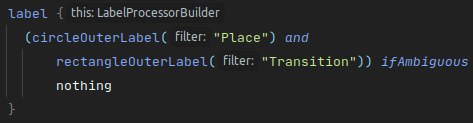
\includegraphics[width=9cm]{images/label-plugin}
\end{frame}


\begin{frame}
  \frametitle{Plugin System}
  \hspace{-1cm}
  \centering
  \includesvg[width=10cm]{images/"presentation - concrete-blur-3"}
\end{frame}

\begin{frame}
  \frametitle{Concrete Syntax Metamodel}
  \hspace{-1cm}
  \centering
  \includesvg[width=10cm]{images/"csd - concretesyntax"}
\end{frame}